% ======================================================================
% POGLAVLJE 4: REZULTATI I DISKUSIJA
% ======================================================================
\chapter{Rezultati i diskusija}
\label{ch:rezultati}

U okviru eksperimentalnog istraživanja sprovedene su ukupno 1.080 planiranih mjernih serija u punom faktorijalnom dizajnu $4 \times 3 \times 3$ (4 konfiguracije $\times$ 3 OLTP/OLAP omjera $\times$ 3 razine konkurentnosti), s 30 serija po kombinaciji. Deset serija (0,93\%) isključeno je iz analize usljed nestabilnosti mjernog okruženja, definisane kao stopa uspješnosti OLTP operacija ispod 90\%. Konačan uzorak obuhvata 1.070 validnih mjerenja, s 28 do 30 serija po svakoj eksperimentalnoj kombinaciji, čime je osigurana statistička pouzdanost provedenih analiza.\footnote{Deskriptivne tabele prikazuju aritmetičke sredine sa standardnom devijacijom radi usporedivosti i čitljivosti. Budući da su distribucije desno-asimetrične (v.\ odjeljak~\ref{sec:statistika}), usporedbe vezane za hipoteze H1 i H3 zasnovane su na medijanima, a svi statistički zaključci na neparametarskim testovima.}

\section{OLAP performanse}
\label{sec:olap_rezultati}

HTAP konfiguracija dominira i u OLAP performansama. Pri $C=32$ HTAP dostiže 6,84 q/s propusnosti, naspram 3,13 q/s za IM, 2,80 q/s za CS i 0,85 q/s za Baseline — poboljšanje od 8,0$\times$ u odnosu na Baseline. Zanimljivo je da IM nadmašuje CS u OLAP propusnosti pri $C=32$ (3,13 vs 2,80 q/s), što ukazuje na kontenciju za memorijskim resursima u batch-mode izvršavanju pri visokoj konkurentnosti.

HTAP postiže najniže OLAP latencije kroz sve omjere opterećenja: $P_{50}=924$\,ms pri 80/20 naspram 3.128\,ms za Baseline (smanjenje od 70\%), odnosno 1.530\,ms pri 20/80 naspram 7.351\,ms za Baseline. Usporedba CS i HTAP pokazuje da je HTAP bolji već pri $C=4$ (825 vs 1.850\,ms, $\Delta=1.025$\,ms, $d=6,14$), a razlika raste pri $C=32$ (1.813 vs 3.620\,ms, $\Delta=1.807$\,ms, $d=6,52$). Distribucija latencija prikazana je na Slikama~\ref{fig:olap_violin_c4}--\ref{fig:olap_violin_c32}.

\begin{figure}[H]
    \centering
    \includegraphics[width=0.85\textwidth]{../Results/figures/02a_olap_violin_c4.png}
    \caption{Distribucija OLAP latencije $P_{50}$ po konfiguracijama -- razina konkurentnosti $C=4$.}
    \label{fig:olap_violin_c4}
\end{figure}

\begin{figure}[H]
    \centering
    \includegraphics[width=0.85\textwidth]{../Results/figures/02b_olap_violin_c16.png}
    \caption{Distribucija OLAP latencije $P_{50}$ po konfiguracijama -- razina konkurentnosti $C=16$.}
    \label{fig:olap_violin_c16}
\end{figure}

\begin{figure}[H]
    \centering
    \includegraphics[width=0.85\textwidth]{../Results/figures/02c_olap_violin_c32.png}
    \caption{Distribucija OLAP latencije $P_{50}$ po konfiguracijama -- razina konkurentnosti $C=32$.}
    \label{fig:olap_violin_c32}
\end{figure}

U Poglavlju~\ref{ch:metodologija} formulirali smo hipotezu H1, čija je suština da disk-zasnovana konfiguracija s columnstore indeksom dostiže usporedivu latenciju analitičkih upita s hibridnom konfiguracijom pri niskim razinama konkurentnosti, dok razlika postaje statistički značajna pri visokim razinama konkurentnih korisnika. Izmjereni podaci to djelimično podupiru, ali ne u potpunosti. Pretpostavka o usporedivosti OLAP latencije CS i HTAP pri niskom $C$ odbačena je: HTAP postiže statistički značajno bolju latenciju \textit{već} pri $C=4$ ($d=6,14$, veliki efekt, $p<0,001$). Razlika iznosi 1.025\,ms pri $C=4$ i raste na 1.807\,ms pri $C=32$, što je konzistentno s modelom u Tabeli~\ref{tab:reg_oba} gdje $\log(\text{Concurrency})$ nosi koeficijent $+0,395$ ($p<0,001$). Hipoteza je dakle potvrđena u svom drugom dijelu -- razlika \textit{raste} s konkurentnošću -- ali odbijena u prvom dijelu koji je pretpostavljao usporedivost pri niskom $C$: in-process dual-store arhitektura HTAP-a pruža prednost nad disk-zasnovanim columnstore pristupom čak i pri minimalnom broju konkurentnih korisnika, jer eliminira I/O latenciju disk-zasnovanog columnstore čitanja. \textbf{Hipoteza H1 je djelimično potvrđena.}

\section{Mješovito opterećenje i degradacija}
\label{sec:misovito_rezultati}

\begin{table}[htbp]
\centering
\caption{Degradacija OLTP propusnosti pri prelasku s 80/20 na 50/50 opterećenje (H2)}
\label{tab:h2}
\small
\begin{tabular}{lrrrl}
\toprule
\textbf{Konfiguracija} & \textbf{Degradacija (\%)} & \textbf{SD (\%)} & \textbf{Cohen's $\bm{d}$} & \textbf{Zaključak} \\
\midrule
CS & 67,4 & 2,8 & 2,315 & potvrđena \\
HTAP & 55,9 & 6,3 & --- & --- \\
\bottomrule
\end{tabular}
\end{table}

CS konfiguracija bilježi degradaciju OLTP propusnosti od 67,4\% pri prelasku s transakcijskog (80/20) na mješovito (50/50) opterećenje, dok HTAP bilježi 55,9\% (Tabela~\ref{tab:h2}). Razlika od 11,5 procentnih poena, uz $p < 0,001$ i $d = 2,315$ (veliki efekt), kvantificira prednost izolacije workloada u dual-store pristupu. Slike~\ref{fig:degrad_c4}--\ref{fig:degrad_c32} prikazuju distribuciju degradacije po konfiguracijama za svaku razinu konkurentnosti.

\begin{figure}[H]
    \centering
    \includegraphics[width=0.85\textwidth]{../Results/figures/05a_oltp_degrad_c4.png}
    \caption{Degradacija OLTP propusnosti pri prelasku s 80/20 na 50/50 omjer opterećenja -- razina konkurentnosti $C=4$.}
    \label{fig:degrad_c4}
\end{figure}

\begin{figure}[H]
    \centering
    \includegraphics[width=0.85\textwidth]{../Results/figures/05b_oltp_degrad_c16.png}
    \caption{Degradacija OLTP propusnosti pri prelasku s 80/20 na 50/50 omjer opterećenja -- razina konkurentnosti $C=16$.}
    \label{fig:degrad_c16}
\end{figure}

\begin{figure}[H]
    \centering
    \includegraphics[width=0.85\textwidth]{../Results/figures/05c_oltp_degrad_c32.png}
    \caption{Degradacija OLTP propusnosti pri prelasku s 80/20 na 50/50 omjer opterećenja -- razina konkurentnosti $C=32$.}
    \label{fig:degrad_c32}
\end{figure}

Slika~\ref{fig:ratio_impact} proširuje analizu na sva tri omjera opterećenja, prikazujući kako HTAP zadržava relativno visoku propusnost čak i pri dominantno analitičkom opterećenju (20\%/80\%).

\begin{figure}[H]
    \centering
    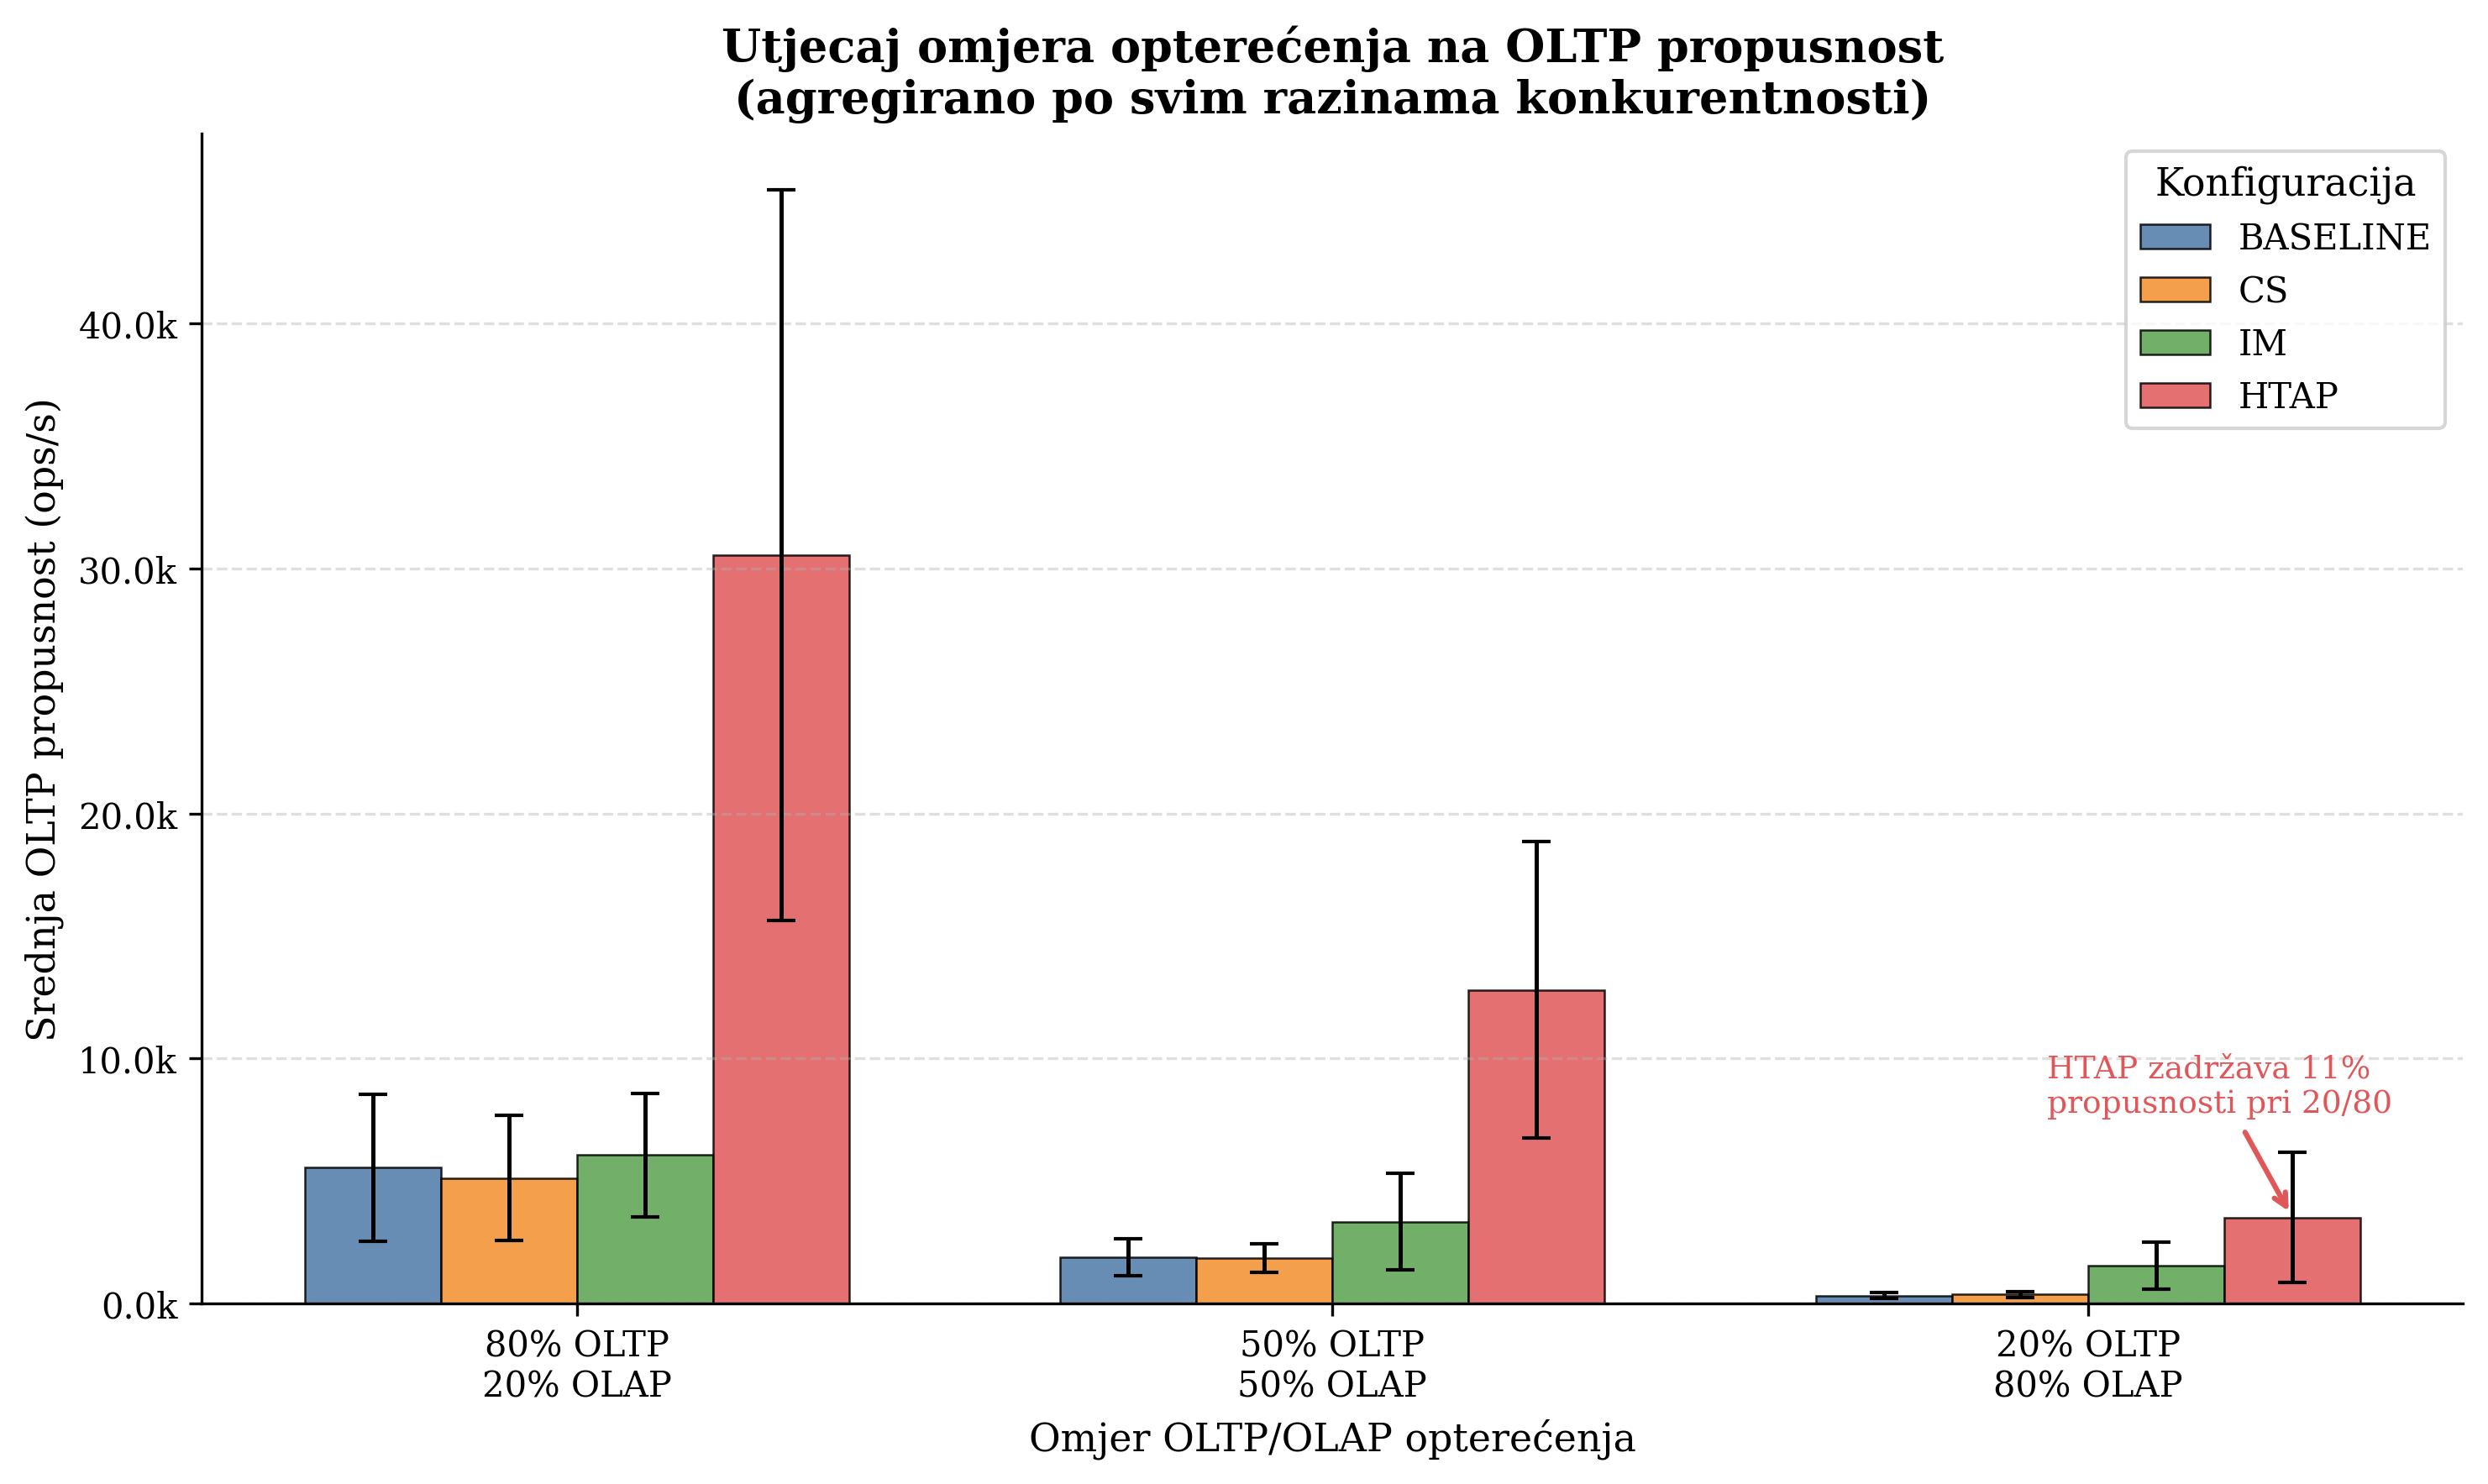
\includegraphics[width=0.85\textwidth]{../Results/figures/12_ratio_impact_bar.png}
    \caption{Uticaj omjera OLTP/OLAP opterećenja na srednju OLTP propusnost (agregirano po svim razinama konkurentnosti). HTAP zadržava relativno visoku propusnost čak i pri dominantno analitičkom opterećenju (20\%/80\%), što potvrđuje izolaciju workloada dual-store mehanizma.}
    \label{fig:ratio_impact}
\end{figure}

U Poglavlju~\ref{ch:metodologija} postavili smo hipotezu H2, prema kojoj je degradacija OLTP propusnosti pri mješovitom opterećenju veća u disk-zasnovanoj konfiguraciji s columnstore indeksom nego u hibridnoj konfiguraciji. Izmjerena degradacija od 67,4\% za CS naspram 55,9\% za HTAP direktno potvrđuje tu pretpostavku. Mehanizam izolacije workloada je jasan: u CS konfiguraciji analitički batch-mode skenovi dijele buffer pool i CPU threadove s OLTP operacijama iz iste disk-zasnovane sheme; u HTAP konfiguraciji analitički upiti čitaju iz \texttt{cs.*} columnstore sloja, dok OLTP operacije koriste \texttt{htap.*} memorijsko-optimizirane tabele koje nikad ne koriste buffer pool -- čime se eliminira primarna tačka međusobne interference. U apsolutnim brojevima, degradacija od 67,4\% pri $C=32$ znači gubitak dvije trećine ukupnog OLTP kapaciteta, što je kritično u scenarijima s ugovorenom razinom usluge (SLA). Ovi nalazi konzistentni su s Wu i drugi \cite{wu2025htap} koji pronalaze degradacijske obrasce od 50 do 70\% za disk-zasnovane sisteme, te sa zaključkom Zhao i drugi \cite{zhao2023benchmarking} da je performansna izolacija pod mješovitim opterećenjem primarni kriterij arhitekturalne kvalitete HTAP sistema. \textbf{Hipoteza H2 je potvrđena} uz statistički značajnu razliku ($p<0{,}001$, $d=2{,}315$ -- veliki efekt).

\section{OLTP performanse}
\label{sec:oltp_rezultati}

HTAP konfiguracija dominira u OLTP propusnosti kroz sve razine konkurentnosti. Pri $C=4$ HTAP postiže 6.783 ops/s, dok IM, CS i Baseline dostižu 2.007, 1.254 i 1.204 ops/s. Pri $C=32$ razlika se dodatno povećava: HTAP dostiže 21.920 ops/s naspram 4.726 ops/s za IM (faktor 4,6$\times$), 2.477 ops/s za CS i 2.432 ops/s za Baseline. Za razliku od memorijsko-optimiziranih konfiguracija, Baseline i CS pokazuju nemonotonu skalabilnost: pri omjeru 80/20 propusnost im opada pri prelasku s $C=16$ na $C=32$ (Baseline 9.005 $\to$ 5.727 ops/s), što je posljedica kontencije za I/O i zaključavanjem pri saturaciji diska.

Pri transakcijsko-intenzivnom opterećenju (80/20 OLTP/OLAP) HTAP nadmašuje IM za faktor koji raste od 3,3$\times$ pri $C=4$ (10.083 vs 3.027\,ops/s, $d=-4,38$) do 6,9$\times$ pri $C=32$ (43.751 vs 6.325\,ops/s, $d=-11,93$).

Slike~\ref{fig:oltp_tl_8020}, \ref{fig:oltp_tl_5050} i~\ref{fig:oltp_tl_2080} prikazuju throughput-latency krivulje za sve četiri konfiguracije, zasebno za svaki omjer OLTP/OLAP opterećenja (80/20, 50/50 i 20/80). Slike~\ref{fig:scalability} i~\ref{fig:update_p95} prikazuju redom skalabilnost propusnosti s porastom broja konkurentnih niti pri omjeru 50/50 te P95 latenciju procedure \texttt{usp\_UpdatePostScore} -- koja u IM konfiguraciji iznosi $11{,}9$\,ms naspram $4{,}3$\,ms u HTAP.

\begin{figure}[H]
    \centering
    \includegraphics[width=0.85\textwidth]{../Results/figures/03a_oltp_tl_8020.png}
    \caption{OLTP Throughput-Latency krivulje po konfiguracijama -- omjer opterećenja 80\%/20\% (pretežno transakcijsko).}
    \label{fig:oltp_tl_8020}
\end{figure}

\begin{figure}[H]
    \centering
    \includegraphics[width=0.85\textwidth]{../Results/figures/03b_oltp_tl_5050.png}
    \caption{OLTP Throughput-Latency krivulje po konfiguracijama -- omjer opterećenja 50\%/50\% (ravnomjerno mješovito).}
    \label{fig:oltp_tl_5050}
\end{figure}

\begin{figure}[H]
    \centering
    \includegraphics[width=0.85\textwidth]{../Results/figures/03c_oltp_tl_2080.png}
    \caption{OLTP Throughput-Latency krivulje po konfiguracijama -- omjer opterećenja 20\%/80\% (pretežno analitičko).}
    \label{fig:oltp_tl_2080}
\end{figure}

\begin{figure}[H]
    \centering
    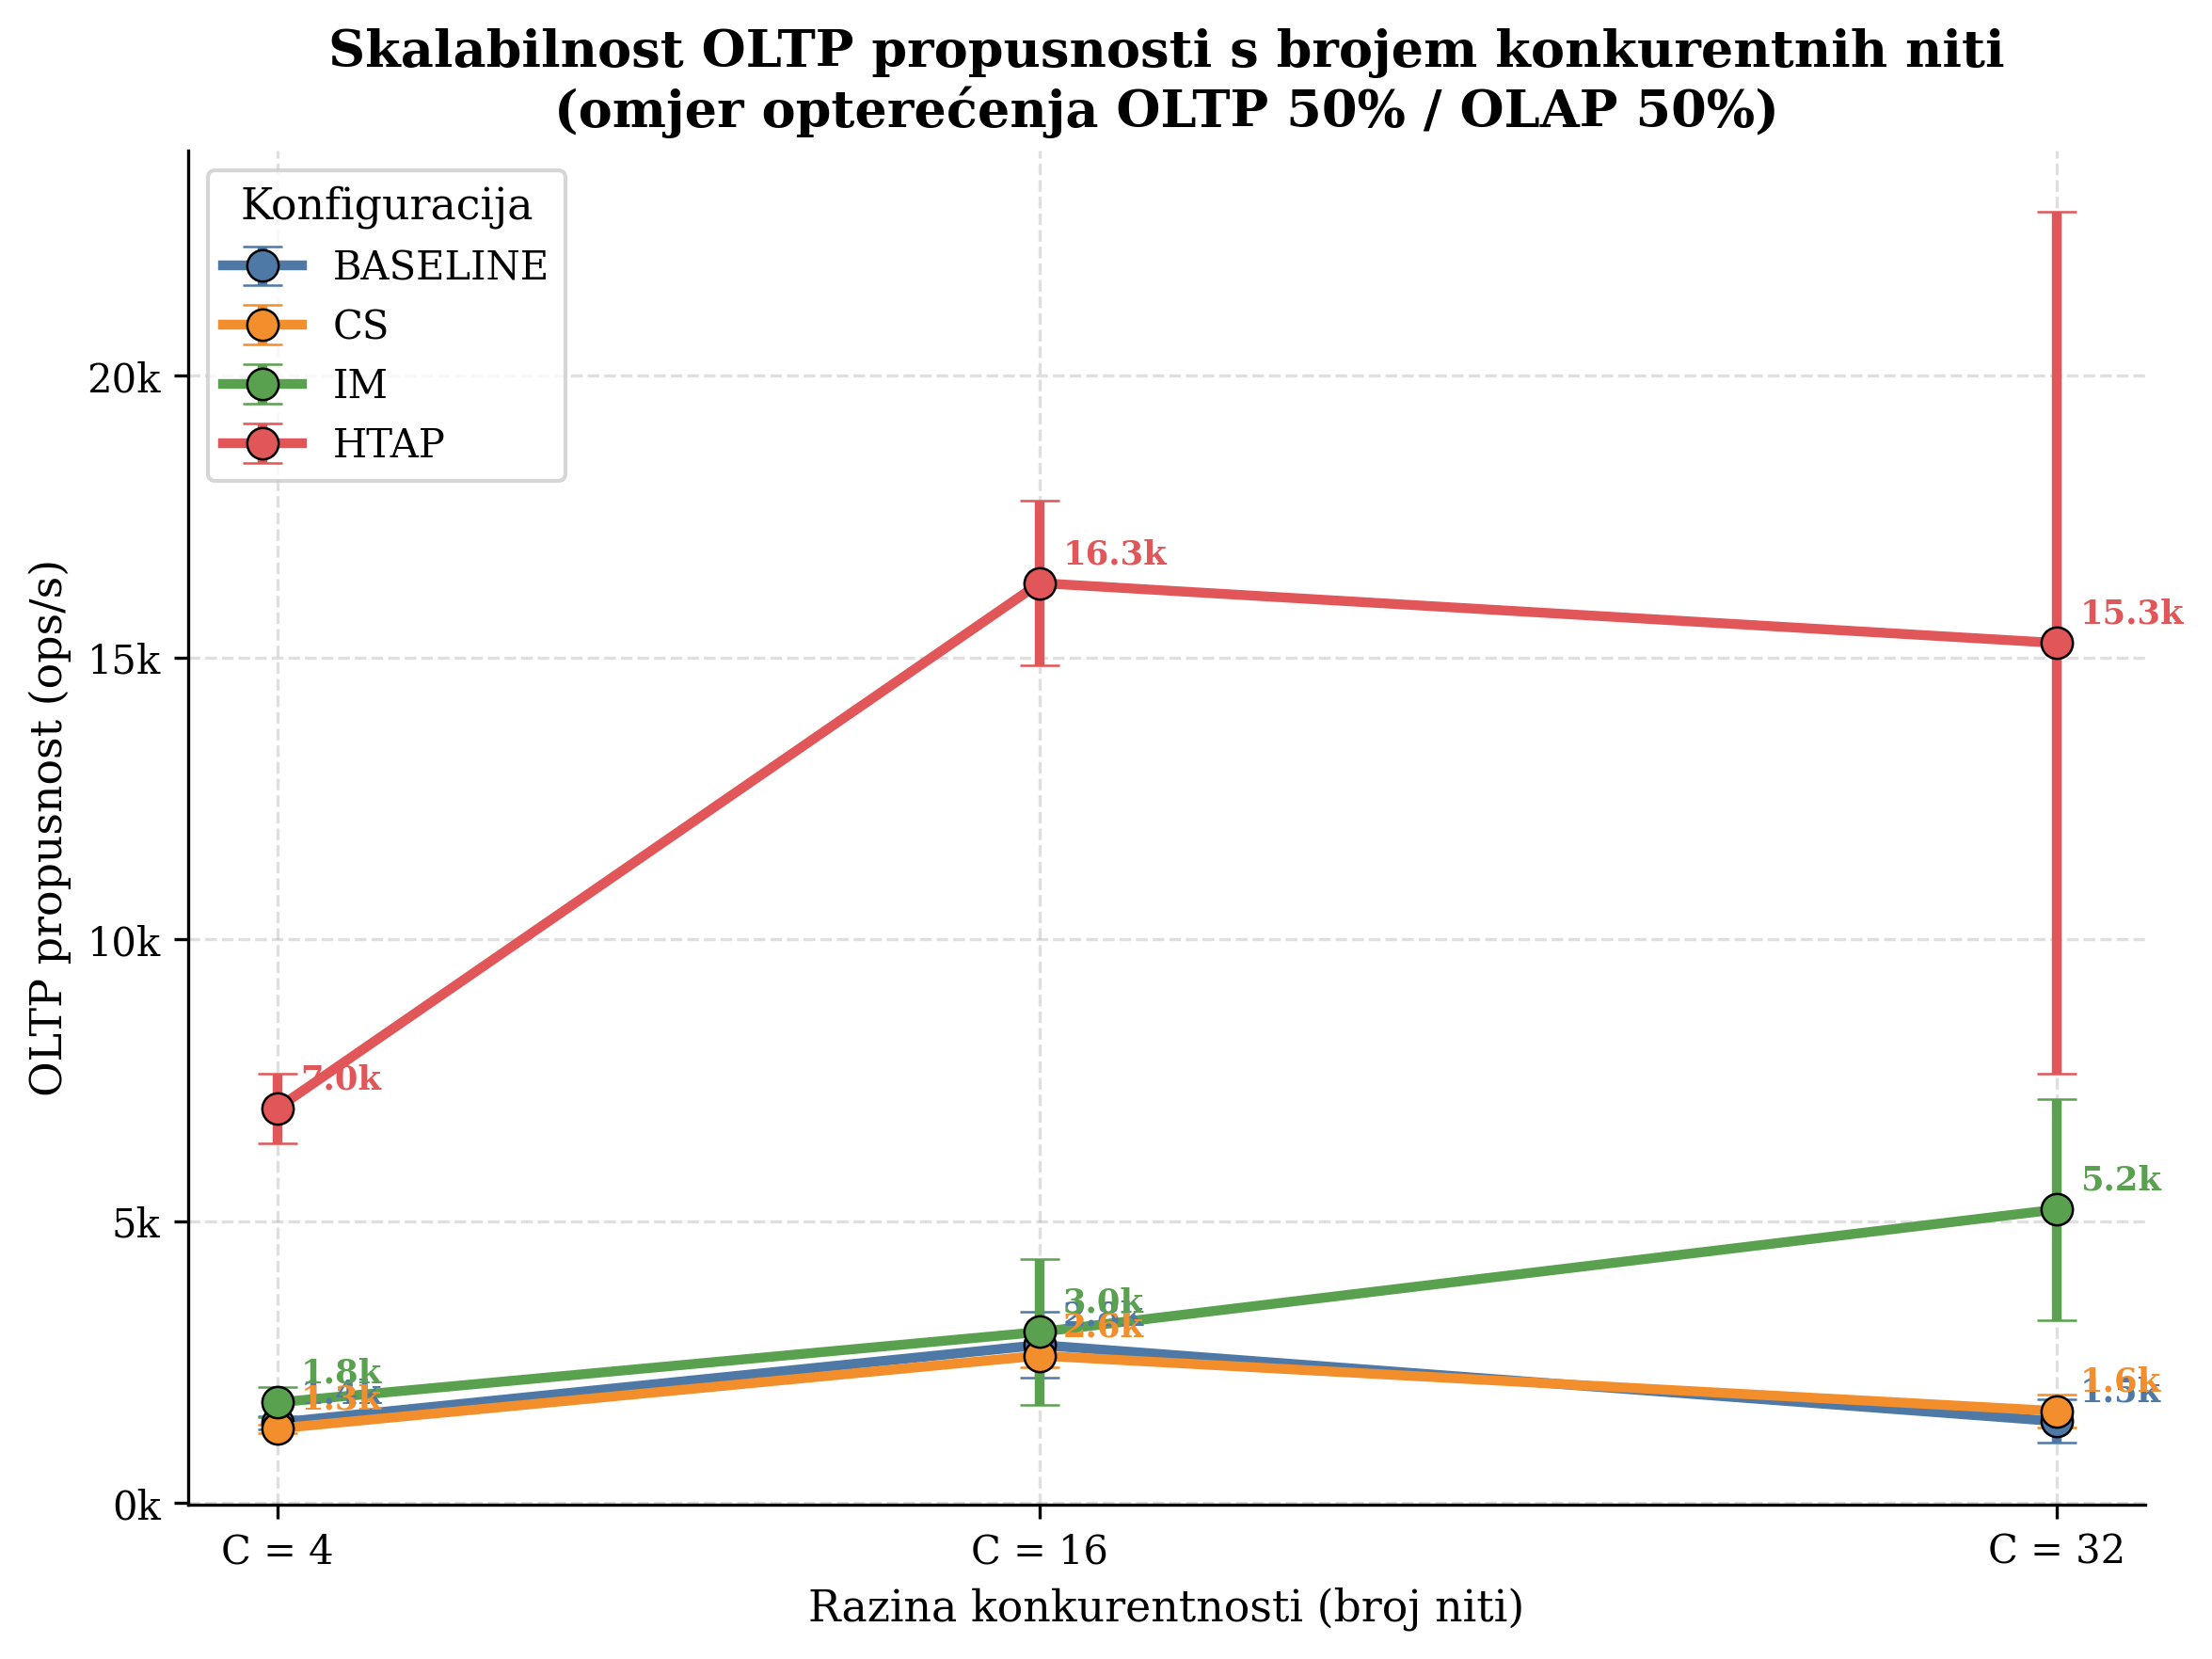
\includegraphics[width=0.85\textwidth]{../Results/figures/11_scalability_line.png}
    \caption{Skalabilnost OLTP propusnosti s brojem konkurentnih niti pri omjeru opterećenja 50\%/50\%. HTAP i IM pokazuju superlinarno povećanje propusnosti pri prelasku s C=4 na C=32, dok Baseline i CS ostaju ograničeni I/O kapacitetom diska.}
    \label{fig:scalability}
\end{figure}

\begin{figure}[H]
    \centering
    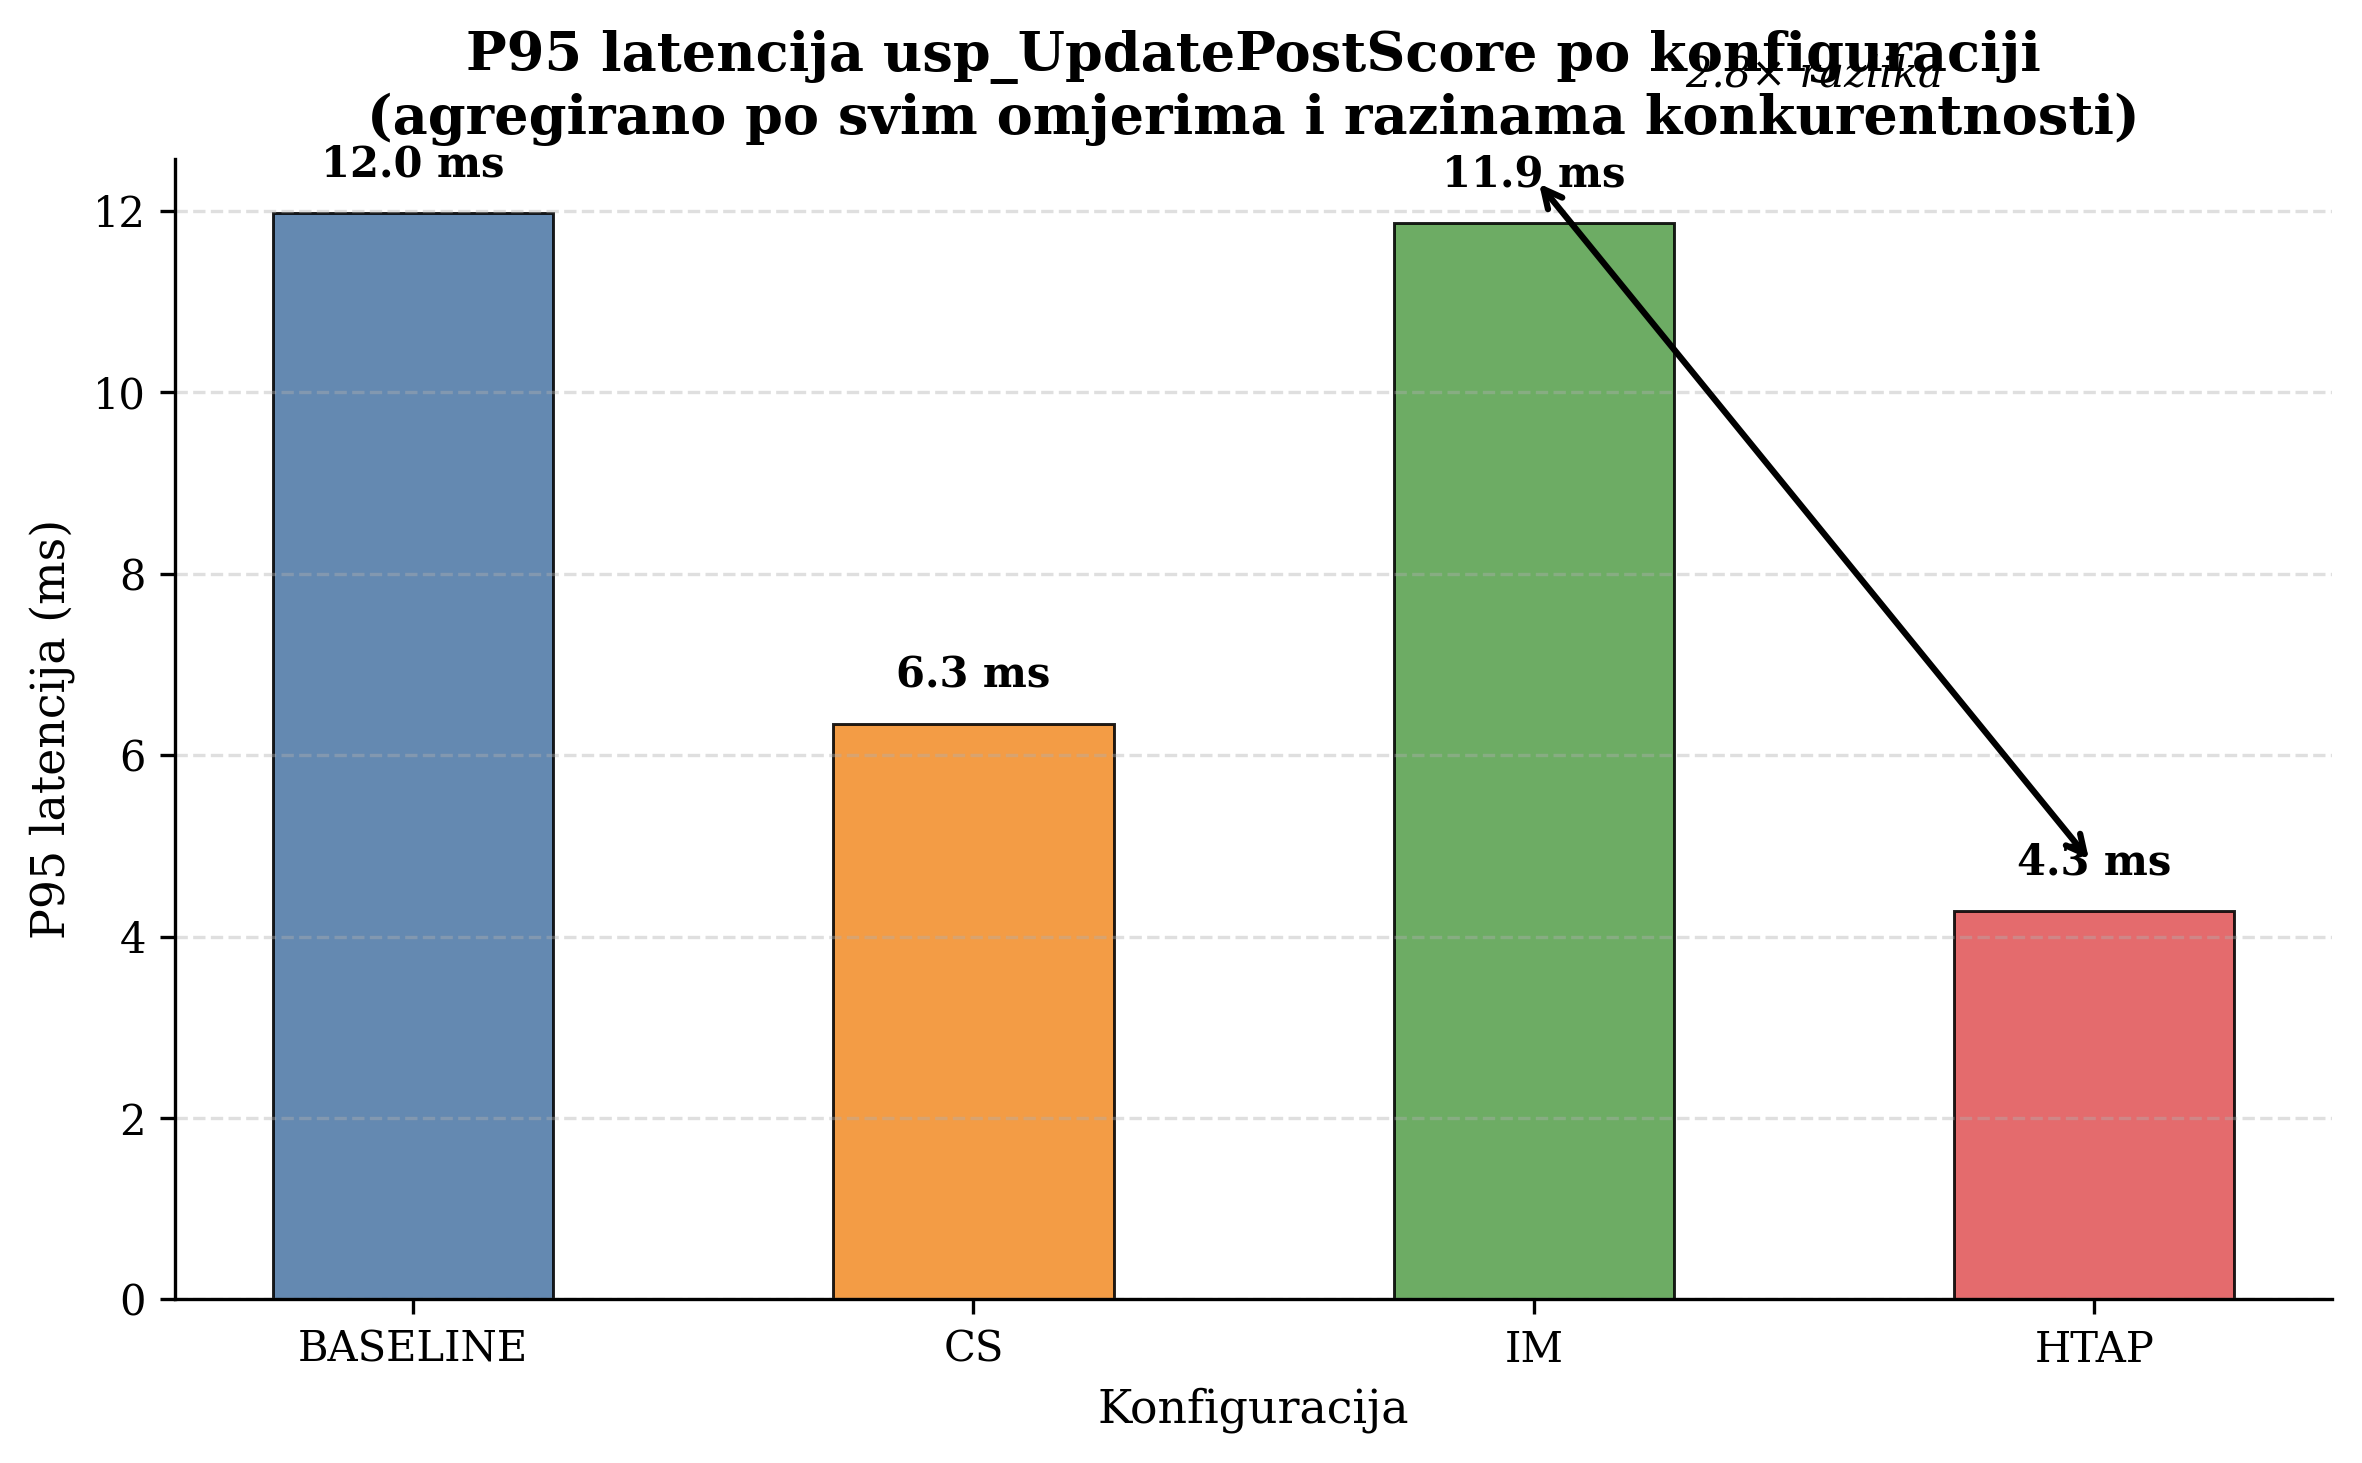
\includegraphics[width=0.85\textwidth]{../Results/figures/13_update_p95_bar.png}
    \caption{P95 latencija procedure \texttt{usp\_UpdatePostScore} po konfiguraciji (agregirano po svim omjerima i razinama konkurentnosti). IM postiže P95\,=\,11,9\,ms naspram HTAP P95\,=\,4,3\,ms -- razlika od 2,8$\times$ pripisuje se, prema modelu izvršavanja upita, CPU saturaciji koju u IM konfiguraciji uzrokuju row-mode OLAP upiti.}
    \label{fig:update_p95}
\end{figure}

U Poglavlju~\ref{ch:metodologija} postavili smo hipotezu H3: hibridna konfiguracija ne ostvaruje statistički značajno veću OLTP propusnost od čisto transakcijske konfiguracije (In-Memory bez columnstore) pri transakcijsko-intenzivnom opterećenju. HTAP ostvaruje 3,3 do 6,9 puta veću OLTP propusnost od IM konfiguracije pri transakcijsko-intenzivnom opterećenju (80/20), s velikim efektima ($d$ od $-4,38$ do $-11,93$) i statističkom značajnošću na svim razinama konkurentnosti ($p < 0,001$, Mann-Whitney U s Bonferroni korekcijom). Mehanizam koji stoji iza ove razlike leži u tipu izvršavanja analitičkih upita: u IM konfiguraciji OLAP upiti rade u row-modu nad memorijsko-optimiziranim tabelama (Hekaton ne podržava batch-mode), čime zasićuju procesorske resurse i direktno natječu s OLTP nitima. U HTAP konfiguraciji columnstore sloj u \texttt{cs.*} shemi ubrzava OLAP za faktor 5--8 i preusmjerava analitička skeniranja dalje od Hekaton memorijskog sloja, čime se OLTP operacije u \texttt{htap.*} shemi izvode bez CPU kompetencije s analitičkim nitima. Napominje se da IM konfiguracija zbog \texttt{CXSYNC\_PORT} čekanja koristi \texttt{MAXDOP 1} za OLAP, dok HTAP koristi \texttt{MAXDOP 2}; ova razlika u stepenu paralelizma analitičkih upita predstavlja confounding varijablu čiji apsolutni doprinos nije izoliran (v.\ odjeljak~\ref{sec:ogranicenja}). \textbf{Hipoteza H3 odbijena je} na svim ispitanim razinama konkurentnosti i svim omjerima opterećenja -- statistički dokazi snažno potvrđuju da HTAP ostvaruje značajno veću OLTP propusnost od IM pri mješovitom opterećenju.

\section{Statistički testovi i regresijska analiza}
\label{sec:statisticki_testovi}

Kruskal-Wallis H-test potvrđuje statistički značajne globalne razlike između konfiguracija za sve mjerne metrike na svim razinama konkurentnosti ($p < 0,001$, df = 3). Najveća H vrijednost zabilježena je za OLTP latenciju $P_{50}$ pri $C=4$ ($H=302,06$) i OLAP propusnost pri $C=16$ ($H=303,17$).

Mann-Whitney U test s Bonferroni korekcijom ($\alpha' = 0,0083$) za OLAP latenciju $P_{50}$ pri $C=32$ pokazuje da su svi parovi konfiguracija statistički značajno različiti ($p < 0,001$ za pet od šest parova, $p = 0,001$ za CS vs IM) s velikim efektima ($|d| > 0,8$) u pet od šest parova, dok par CS--IM pokazuje srednji efekt ($d = 0,679$).

Uz neparametarsku analizu, provedena je i parametarska analiza radi kvantifikacije veličine efekta faktora i izgradnje prediktivnog modela performansi. Konstruirana su dva OLS regresijska modela s logaritamskom transformacijom zavisnih varijabli:

\begin{align}
\log(\text{OltpThroughput}) &\sim \text{Config} + \text{OltpOlapRatio} + \log(\text{Concurrency}) \label{eq:oltp_reg} \\
\log(\text{OlapLatencyP50}) &\sim \text{Config} + \text{OltpOlapRatio} + \log(\text{Concurrency}) \label{eq:olap_reg}
\end{align}

\begin{table}[htbp]
\centering
\caption{OLS regresijski koeficijenti za oba modela ($N=1.065$; sve vrijednosti $p<0{,}001$ osim CS za OLTP)}
\label{tab:reg_oba}
\small
\begin{tabular}{lrrrr}
\toprule
 & \multicolumn{2}{c}{\textbf{log(OltpThroughput)}} & \multicolumn{2}{c}{\textbf{log(OlapLatencyP50)}} \\
\cmidrule(lr){2-3}\cmidrule(lr){4-5}
\textbf{Parametar} & Koef. & $p$ & Koef. & $p$ \\
\midrule
CS vs Baseline        &  0,021 & 0,600 & $-0,636$ & $<0,001$ \\
IM vs Baseline        &  0,708 & $<0,001$ & $-1,166$ & $<0,001$ \\
\textbf{HTAP vs Baseline} & \textbf{1,965} & $<\mathbf{0,001}$ & $\mathbf{-1,382}$ & $<\mathbf{0,001}$ \\
Omjer 50/50 vs 80/20  & $-0,821$ & $<0,001$ & $+0,403$ & $<0,001$ \\
Omjer 20/80 vs 80/20  & $-2,211$ & $<0,001$ & $+0,640$ & $<0,001$ \\
$\log(\text{Concurrency})$ & $+0,325$ & $<0,001$ & $+0,395$ & $<0,001$ \\
\midrule
$R^2$ & \multicolumn{2}{c}{0,881} & \multicolumn{2}{c}{0,854} \\
\bottomrule
\end{tabular}
\end{table}

Koeficijent HTAP konfiguracije u modelu~\eqref{eq:oltp_reg} iznosi $+1,965$ ($p<0,001$), što znači da HTAP ima $e^{1,965} \approx 7,14$ puta veću OLTP propusnost od Baseline ($R^2 = 0,881$). U modelu~\eqref{eq:olap_reg} koeficijent $-1,382$ odgovara smanjenju OLAP latencije za faktor $e^{1,382} \approx 3,98$ u korist HTAP ($R^2 = 0,854$).

\section{Interpretacija rezultata i usporedba s literaturom}
\label{sec:interpretacija}

Izmjereni rezultati otkrivaju fundamentalni mehanizam dual-store arhitekture koji do sada nije bio eksplicitno kvantificiran u nezavisnoj literaturi: columnstore sloj ne samo da ubrzava analitičke upite, već indirektno štiti transakcijske resurse od analitičke interference. Ovaj mehanizam objašnjava zašto HTAP nadmašuje ne samo disk-zasnovane konfiguracije, već i memorijsko-optimiziranu IM konfiguraciju koja koristi isti Hekaton engine.

U IM konfiguraciji OLAP upiti izvode full-table skenove nad hash indeksima memorijsko-optimiziranih tabela u row-modu, zahtijevajući znatno više CPU ciklusa po redu i dovodeći do saturacije procesora pri visokim razinama konkurentnosti ($C=16$, $C=32$). U HTAP konfiguraciji columnstore indeksi u \texttt{cs.*} sloju ubrzavaju OLAP za faktor 5--8 (batch-mode naspram row-mode), dok OLTP operacije u \texttt{htap.*} sloju nikada ne dijele CPU s analitičkim nitima. Poboljšanje OLAP performansi nije samo cilj sam po sebi -- ono je i sredstvo za zaštitu OLTP propusnosti.

Zanimljiv je i nalaz da IM (3,13\,q/s) nadmašuje CS (2,80\,q/s) u OLAP propusnosti pri $C=32$, unatoč tome što CS posjeduje columnstore indekse. Objašnjenje leži u kontenciji za memorijskim resursima pri visokoj konkurentnosti: pri $C=32$ sa 6 i više simultanih batch-mode upita, čekanje na dodjelu memorijskog prostora (\texttt{RESOURCE\_SEMAPHORE}) povećava ukupno trajanje izvršavanja više nego što ga batch-mode skraćuje. IM konfiguracija, s podacima potpuno u RAM-u i bez batch-mode overhead-a, izbjegava taj problem, što je konzistentno sa Zeng i drugi \cite{zeng2023empirical}.

\textbf{Usporedba s literaturom.} Zhang i drugi \cite{zhang2024htap} tvrde da dual-engine sistemi imaju bolju izolaciju, ali plaćaju mrežnu latenciju -- SQL Server-ov in-process dual-store empirijski potvrđuje bolju izolaciju uz eliminaciju mrežne latencije. Zhao i drugi \cite{zhao2023benchmarking} ističu performansnu izolaciju kao primarni kriterij arhitekturalne kvalitete, što ovaj rad potvrđuje: CS degradacija od 67,4\% naspram HTAP-ove 55,9\% konkretno ilustruje tu razliku. Wu i drugi \cite{wu2025htap} pronalaze degradacijske obrasce od 50 do 70\% za disk-zasnovane sisteme, što je konzistentno s izmjerenih 67,4\% za CS konfiguraciju. Odbacivanje H3 kvantificira efekt koji dosad nije bio eksplicitno izmjeren: columnstore ubrzanje OLAP-a ima pozitivan indirektan uticaj na OLTP propusnost pri mješovitom opterećenju.

\section{Završna razmatranja}
\label{sec:preporuke}
\label{sec:ogranicenja}

Na osnovu empirijskih nalaza, HTAP dual-store konfiguracija preporučuje se za sve scenarije s mješovitim OLTP/OLAP opterećenjem (Tabela~\ref{tab:preporuke}). CS ostaje relevantan za isključivo analitičke workloade ili okruženja s ograničenim RAM-om. Baseline nije preporučen za produkcijska okruženja s analitičkim zahtjevima.

\begin{table}[htbp]
\centering
\caption{Praktične preporuke za odabir konfiguracije u SQL Serveru 2022}
\label{tab:preporuke}
\small
\begin{tabular}{>{\raggedright\arraybackslash}p{4.5cm}>{\centering\arraybackslash}p{3cm}>{\raggedright\arraybackslash}p{5.5cm}}
\toprule
\textbf{Scenario} & \textbf{Preporuka} & \textbf{Empirijska osnova} \\
\midrule
$>80\%$ OLTP, $<20\%$ OLAP & HTAP & 3,3--6,9$\times$ veća OLTP propusnost; OLAP $P_{50}=924$\,ms \\
50--80\% OLTP, 20--50\% OLAP & HTAP & Najniža OLTP degradacija (55,9\%) i OLAP latencija \\
$<50\%$ OLTP, $>50\%$ OLAP & HTAP & OLAP $P_{50}=1.530$\,ms vs 3.710\,ms za CS \\
Samo OLAP, bez transakcija & CS & 7$\times$ bolja OLAP propusnost vs Baseline \\
RAM ograničen ili SQL Express & CS & Express ne podržava In-Memory OLTP \\
\bottomrule
\end{tabular}
\end{table}

Preporuke u Tabeli~\ref{tab:preporuke} odnose se isključivo na performanse i pretpostavljaju da su zadovoljeni preduslovi dual-store pristupa: otprilike dvostruka potrošnja RAM-a (podaci u Hekaton sloju plus columnstore kopija), inženjerski trošak izgradnje i održavanja sinhronizacije između \texttt{htap.*} i \texttt{cs.*} slojeva (koji benchmark ne mjeri) te tolerancija aplikacije na analitiku nad podacima koji nisu svježi u realnom vremenu. U scenarijima gdje ti preduslovi nisu zadovoljeni, CS konfiguracija predstavlja pragmatičan kompromis.

Rezultate ovog rada treba tumačiti u svjetlu nekoliko ograničenja.

Ispitana HTAP konfiguracija fizički odvaja OLTP sloj (\texttt{htap.*}) od analitičkog sloja (\texttt{cs.*}), ali tokom mjerenja ne radi nikakav mehanizam sinhronizacije (CDC, replikacija ili kompakcija) koji bi održavao svježinu analitičke kopije. Produkcijski dual-store sistemi plaćaju kontinuiranu cijenu te sinhronizacije -- TiDB Raft replikaciju na learner čvorove \cite{huang2020tidb}, F1 Lightning Changepump i četiri vrste kompakcije \cite{yang2020f1}. Izmjerene prednosti (3,3--6,9$\times$ nad IM, najniža degradacija) stoga predstavljaju gornju granicu ostvarivu uz nultu cijenu sinhronizacije i analitiku nad podacima koji nisu svježi u realnom vremenu, pa rad kvantificira koliko interferencije uklanja fizička separacija slojeva, a ne neto dobit produkcijski potpuno konzistentnog dual-store sistema.

\looseness=-1
Memorijsko-optimizirane konfiguracije (IM, HTAP) koriste \texttt{DURABILITY\allowbreak{} =\allowbreak{} SCHEMA\_ONLY}, čime se eliminira pisanje u transakcijski log; u produkciji s \texttt{SCHEMA\_AND\_DATA} durabilnošću OLTP propusnost bila bi niža, a jaz prema disk-zasnovanim konfiguracijama manji. Disk-zasnovane konfiguracije (Baseline, CS) rade na NVMe SSD-u, dok IM/HTAP čitaju iz RAM-a, pa multiplikatori koji uspoređuju konfiguracije između različitih medija miješaju efekt arhitekture s efektom medija i durabilnosti. Usporedbe unutar istog medija i durabilnosti -- HTAP naspram IM (H3) te CS naspram HTAP analitičkog sloja (H1) -- metodološki su najčistije.

Analitičke procedure koriste \texttt{MAXDOP 2} na CS/HTAP, a \texttt{MAXDOP 1} na IM zbog \texttt{CXSYNC\_PORT} čekanja na Hekaton tabelama. Ova tehnički nužna razlika u stepenu paralelizma analitičkih upita predstavlja confounding varijablu u usporedbi H3 (HTAP vs IM): izmjereni jaz u OLTP propusnosti dijelom reflektira razliku u stepenu paralelizma, a ne isključivo dual-store arhitekturu, pri čemu apsolutni doprinos ove asimetrije nije kvantificiran.

Objašnjenje prednosti HTAP-a nad IM-om počiva na CPU saturaciji uzrokovanoj row-mode skeniranjem, ali taj mehanizam izveden je iz modela izvršavanja upita, a ne iz direktnog profilisanja procesora koje nije instrumentirano. Direktno mjerenje CPU iskorištenosti po konfiguraciji ostaje predmet budućeg rada.

Sva mjerenja provedena su na jednoj instanci SQL Servera 2022 nad jednim skupom podataka (StackOverflow2010). Generalizacija na distribuirane sisteme, druge skupove podataka ili buduće verzije DBMS-a zahtijeva oprez, a nije isključena blaga autokorelacija usljed stanja buffer pool-a između sekvencijalno izvršavanih serija iste kombinacije.
